\documentclass{beamer}
\usepackage[utf8]{inputenc}
\usepackage{graphicx}
\usepackage{hyperref}

\title{Summer 2018 Recruitment Slide Deck}

\newcommand{\pic}[1]{ \begin{frame}\includegraphics[width=\textwidth]{#1}\end{frame} }

\begin{document}

\begin{frame}
  \textbf{\LARGE Family Support Center of South Sound}\\
  {\Large Community Service \& Volunteerism, Summer 2018}\\
  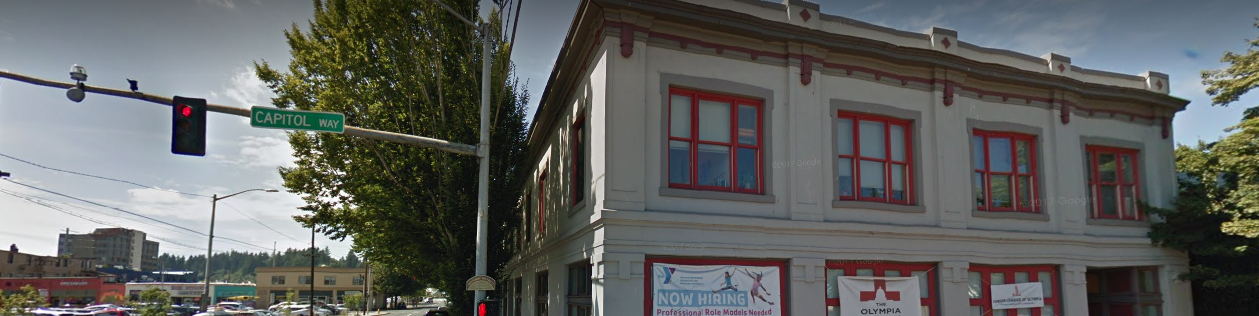
\includegraphics[width=\textwidth]{main-office.png}
\end{frame}

\begin{frame}
  \begin{figure}
  \centering
    \begin{minipage}{0.49\textwidth}
    \centering
    \includegraphics[origin=c,angle=270,width=\textwidth]{holidays.jpg} 
    \end{minipage}\hfill
    \begin{minipage}{0.49\textwidth}
    \centering
    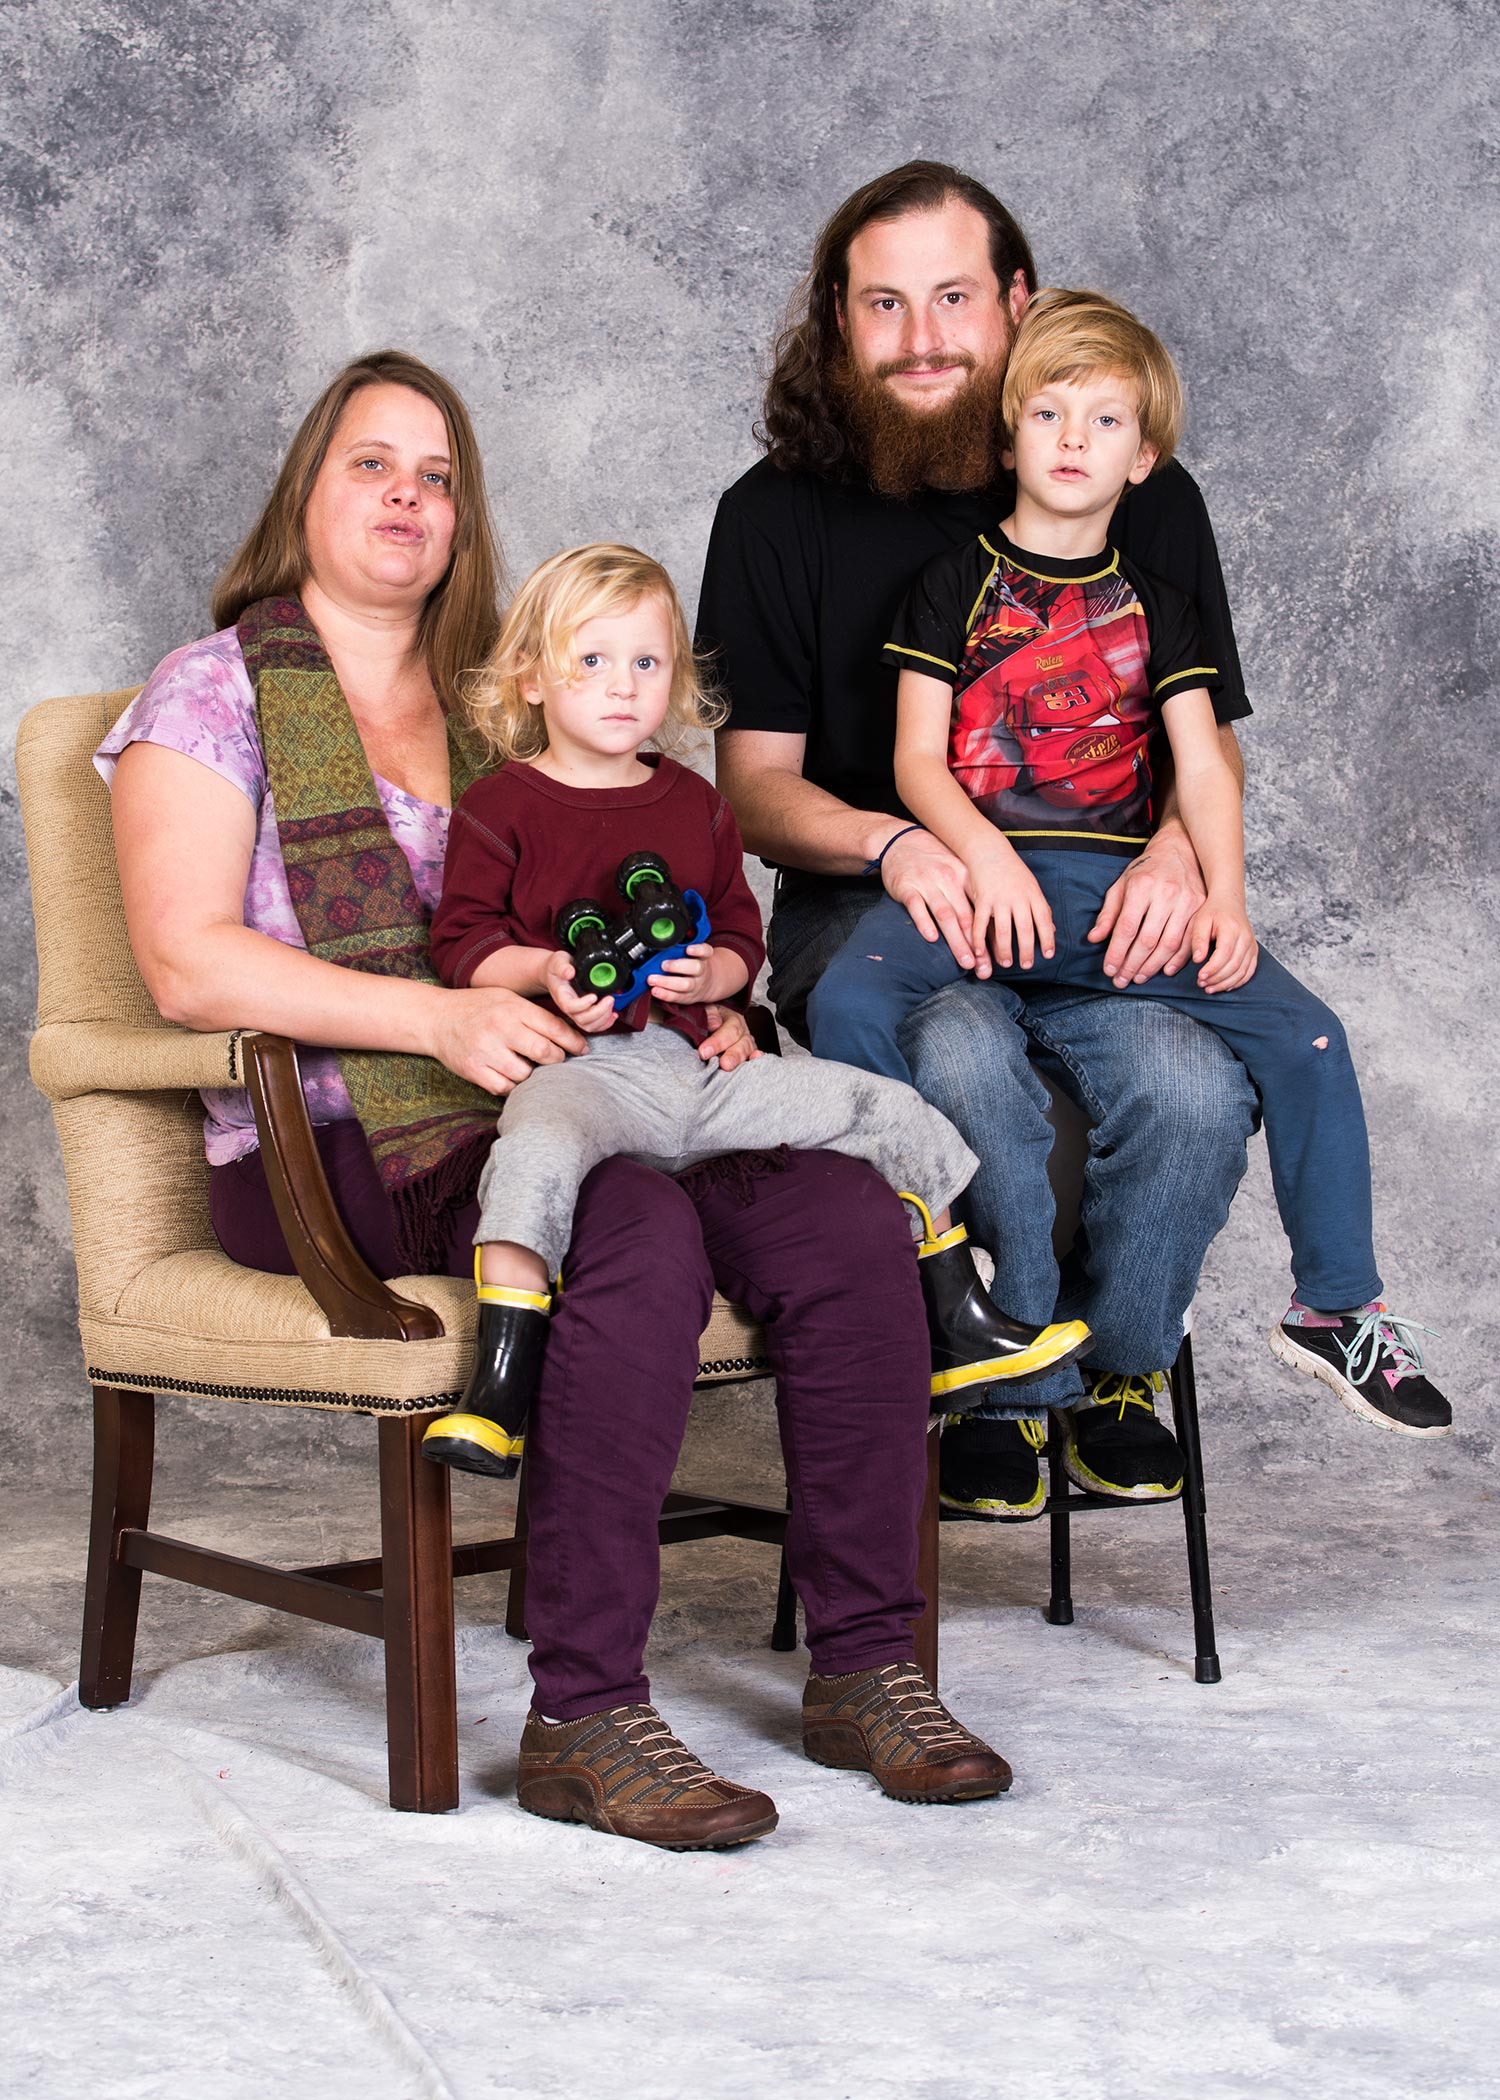
\includegraphics[width=\textwidth]{portrait-family.jpg}
    \end{minipage}
  \end{figure}
\end{frame}

\pic{pear-blossom.jpg}
\pic{living-room.jpg}
\pic{donation-room.jpg}
\pic{snow.jpg}
\pic{straddle.jpg}
\pic{portrait.jpg}

\begin{frame}
  \textbf{\LARGE How to get started}\\
  \begin{enumerate}
    \item Apply at \url{volunteer.fscss.org}.
    \item Schedule an orientation.
    \item Complete training parts A and B.
  \end{enumerate}
\end{frame}

\end{document}

